%% LaTeX2e class for student theses
%% thesis.tex
%% 
%% Karlsruhe Institute of Technology
%% Institute for Program Structures and Data Organization
%% Chair for Software Design and Quality (SDQ)
%%
%% Dr.-Ing. Erik Burger
%% burger@kit.edu
%%
%% Version 1.3.3, 2018-04-17

%% Available page modes: oneside, twoside
%% Available languages: english, ngerman
%% Available modes: draft, final (see README)

\documentclass[twoside, english, draft]{sdqthesis}
\usepackage{amsmath}
\usepackage{graphicx}
\usepackage{algorithm}
\usepackage{algpseudocode}
\usepackage{subcaption}
\usepackage{graphicx}

\graphicspath{
	{images/}
}
\setlength{\parindent}{0em}
\setlength{\parskip}{1em}

\algnewcommand\algorithmicforeach{\textbf{for each}}
\algdef{S}[FOR]{ForEach}[1]{\algorithmicforeach\ #1\ \algorithmicdo}

\usepackage{hyperref}
\hypersetup{
	colorlinks=true,
	linkcolor=blue,
	filecolor=magenta,      
	urlcolor=cyan,
}

%% ---------------------------------
%% | Information about the thesis  |
%% ---------------------------------

%% Name of the author
\author{Beini Ma}

%% Title (and possibly subtitle) of the thesis
\title{Importance Sampling in Many Lights Trees}

%% Type of the thesis 
\thesistype{Bachelor's Thesis}

%% Change the institute here, ``IPD'' is default
\myinstitute{Computer Graphics Group}

%% You can put a logo in the ``logos'' directory and include it here
%% instead of the SDQ logo
% \grouplogo{myfile}
%% Alternatively, you can disable the group logo
\nogrouplogo

%% The reviewers are the professors that grade your thesis
\reviewerone{Prof. Dr.-Ing. Carsten Dachsbacher}
\reviewertwo{Prof. B}

%% The advisors are PhDs or Postdocs
\advisorone{M.Sc. Alisa Jung}

%% Please enter the start end end time of your thesis
\editingtime{23. April 2018}{23. August 2018}

\settitle

%% --------------------------------
%% | Settings for word separation |
%% --------------------------------

%% Describe separation hints here.
%% For more details, see 
%% http://en.wikibooks.org/wiki/LaTeX/Text_Formatting#Hyphenation
\hyphenation{
	% me-ta-mo-del
}

%% --------------------------------
%% | Bibliography                 |
%% --------------------------------

%% Use biber instead of BibTeX, see README
\usepackage[citestyle=numeric,style=alphabetic,backend=biber]{biblatex}
\addbibresource{thesis.bib}

%% ====================================
%% ====================================
%% ||                                ||
%% || Beginning of the main document ||
%% ||                                ||
%% ====================================
%% ====================================
\begin{document}
	
	%% Set PDF metadata
	\setpdf
	
	%% Set the title
	\maketitle
	
	%% The Preamble begins here
	\frontmatter
	
	%% LaTeX2e class for student theses: Declaration of independent work
%% sections/declaration.tex
%% 
%% Karlsruhe Institute of Technology
%% Institute for Program Structures and Data Organization
%% Chair for Software Design and Quality (SDQ)
%%
%% Dr.-Ing. Erik Burger
%% burger@kit.edu
%%
%% Version 1.3.3, 2018-04-17

\thispagestyle{empty}
\null\vfill
\noindent\hbox to \textwidth{\hrulefill} 
\iflanguage{english}{I declare that I have developed and written the enclosed
thesis completely by myself, and have not used sources or means without
declaration in the text.}%
{Ich versichere wahrheitsgemäß, die Arbeit
selbstständig angefertigt, alle benutzten Hilfsmittel vollständig und genau
angegeben und alles kenntlich gemacht zu haben, was aus Arbeiten anderer
unverändert oder mit Änderungen entnommen wurde.}
 
 
%% ---------------------------------------------
%% | Replace PLACE and DATE with actual values |
%% ---------------------------------------------
\textbf{Karlsruhe, 23. August 2018}
\vspace{1.5cm}
 
\dotfill\hspace*{8.0cm}\\
\hspace*{2cm}(\theauthor) 
\cleardoublepage
	
	\setcounter{page}{1}
	\pagenumbering{roman}
	
	%% ----------------
	%% |   Abstract   |
	%% ----------------
	
	%% For theses written in English, an abstract both in English
	%% and German is mandatory.
	%%
	%% For theses written in German, a German abstract is sufficient.
	%%
	%% The text is included from the following files:
	%% - sections/abstract
	
	\includeabstract
	
	%% ------------------------
	%% |   Table of Contents  |
	%% ------------------------
	\tableofcontents
	
	\listoffigures
	
	%% -----------------
	%% |   Main part   |
	%% -----------------
	
	\mainmatter
	
	%% LaTeX2e class for student theses
%% sections/content.tex
%% 
%% Karlsruhe Institute of Technology
%% Institute for Program Structures and Data Organization
%% Chair for Software Design and Quality (SDQ)
%%
%% Dr.-Ing. Erik Burger
%% burger@kit.edu
%%
%% Version 1.3.3, 2018-04-17

\chapter{Introduction}
\label{ch:Introduction}

\section{Problem/Motivation}
\label{sec:Introduction:Motivation}

Ray tracing is one of the most important rendering techniques when the aim is to create highly realistic pictures. It allows us to render the scene much closer to reality compared to typical scanline rendering methods at the cost of more computations. In situations where the images can be rendered ahead of time, such as for visual effects or films, we can take advantage of the better results of ray tracing. Then again, ray tracing is not useful for real-time applications like video games where the rendering speed is critical. But even when it comes to ray tracing, we cannot completely ignore the rendering time. Too long rendering times are becoming a problem in scenes with many lights. For instance a scene of big city with skyscrapers at night could have hundreds or thousands of lights that could potentially all affect a single point in the scene. Typical light sampling methods would be too slow to deal with these situations, since we cannot calculate the effect of every single light on the sampled point.\cite{PBR}\cite{MLA}\cite{MLS}\cite{LCT}

There are sampling approaches that try to limit the time required to render these scenes with a big amount of lights. For instance, we could say that the probability of a point of the scene being sampled by a certain light is only dependent on the emission power of said light. We would make a distribution that only takes into account the emission power of the lights. To light a point we would then pick out a single light with a random number generator and sample the point with that light. Obviously there are a lot of problems with this approach. An area light source or a spotlight could be facing towards a completely different direction and not have any effect on the point. Or the light could be potentially too far away to have a noticeable effect on the point. This sampling technique asserts a fast sampling speed but can lead to very noisy images that we try to avoid.

For this bachelor thesis I have implemented a light sampling technique that optimizes the rendering speed without making the rendered image too noisy.

\section{Content}
\label{sec:Introduction:Content}
	%% LaTeX2e class for student theses
%% sections/content.tex
%% 
%% Karlsruhe Institute of Technology
%% Institute for Program Structures and Data Organization
%% Chair for Software Design and Quality (SDQ)
%%
%% Dr.-Ing. Erik Burger
%% burger@kit.edu
%%
%% Version 1.3.3, 2018-04-17

\chapter{Preliminaries}
\label{ch:preliminaries}

\section{Probability Theory Basics}
\label{ch:preliminaries:ptb}

In this section we will be discussing basic ideas and define certain terms from the probability theory. We will assume that the reader is already familiar with most of the concepts and therefore will only give a short introduction. If the reader struggles following the key parts of this section, he is heavily advised to read more extensive literature about this subject. We suggest E. T. Jaynes \textit{Probability Theory: The Logic of Science} for this matter. \cite{PTTLS}

\subsection{Random Variable}

A random variable $X$ is a variable whose values are numerical outcomes chosen by a random process. There are discrete random variables, which can only take a countable set of possible outcomes and continuous random variables with an uncountable number of possible results. For instance, flipping a coin would be a random variable drawn from a discrete domain which can only result to heads or tails, while sampling a random direction over a unit sphere can produce infinite different directions. In rendering and particularly in path tracing, we are often sampling certain directions or light sources in order to illuminate the scene, therefore we will be handling both discrete and continuous random variables, albeit with the latter in the most cases.

The so-called canonical uniform random variable $\xi$ is a special continuous random variable that is especially important for us. Every interval in its domain [0, 1) with equal length are assigned the same probability. This random variable makes it very easy to generate samples from arbitrary distributions. For example, if we would need to sample a direction to estimate the incident lighting on a point, we could draw two samples from $\xi$ and scale these two values with appropriate transformations so they reflect the polar coordinates of direction to sample.

\subsection{Probability Density Function}

For continuous random variables, probability density functions (PDF) illustrate how the possible outcomes of the random experiment are distributed across the domain. They must be nonnegative and integrate to 1 over the domain. $p:D \rightarrow \mathbb{R}$ is a PDF when
\begin{equation}
\int_{D}p(x)\mathrm{d}x = 1.
\end{equation}
Integrating over a certain interval $[a, b]$ gives the possibility that the random experiment returns a result that lies inside of given interval:
\begin{equation}
\int_{a}^{b}p(x)\mathrm{d}x = P(x \in [a, b])
\end{equation}
It is evident, that $P(x \in [a, a]) = 0$ which reflects the fundamental idea of continuous random variables: The possibility of getting a sample that exactly equals a certain number is zero. Therefore, PDFs are only meaningful when regarded over a interval and not over a single point.

\subsection{Expected Values and Variance}

As the name already indicates, the expected value $E_p[f(x)]$ of a function $f$ and a distribution $p$ specifies the average value of the function after getting a large amount of samples according to the distribution function $p(x)$. Over a certain domain $D$, the expected value is defined as
\begin{equation}
E[f(x)] = \int_{D}f(x)p(x)\mathrm{d}x.
\end{equation}

The variance defines a measure that illustrates the distance between the actual sample values and their average value. Formally, it is defined by the expectation of the squared deviation of the function from its expected value:
\begin{equation}
V[f(x)] = E[(f(x) - E[f(x)])^2]
\end{equation}
When we talk about Monto Carlo Intergration later, the variance is a strong indicator of the quality of the PDF we chose. The main part of this thesis will be to minimize the variance of light sampling methods.

\subsection{Error and Bias} 

For an estimator $F_N$, the parameter to be estimated $I$ and a sample $x$ the error $e(x)$ is defined as

\begin{equation}
e(x) = F_N(x) - I.
\end{equation}

Since the error is dependent on the certain sample we took, we will also introduce bias. The bias $b$ of an estimator is the expected value of the error:

\begin{equation}
b(F_N) = E[F_N - I].
\end{equation}

An estimator $F_N$ is unbiased, if $b(F_N) = 0$ for all sample sizes N. Informally, it means that the estimator is going to return the correct value on average. In the next section, we will introduce an unbiased estimator, the Monte Carlo estimator.

\section{Monte Carlo Integration}
\label{ch:preliminaries:mci}

When generating an image using path tracing, we will be dealing with integrals and our main task will be to estimate the values of these integrals. Since they are almost never available in closed form, like the incident lighting of a certain point that theoretically requires infinite number of rays traced over infinite dimensions, analytical integration methods do not work. Instead, we have to use numerical integration methods give an appropriate estimation for these integrals. One of the most powerful tools we have in this regard is the Monto Carlo integration. We will be discussing the advantages of Monte Carlo integration, as well as its constraints and mechanisms how we can deal with these limits.

Using random sampling methods, we want to evaluate the integral 

\begin{equation}
I = \int_{a}^{b}f(x)d(x)
\end{equation}

with Monte Carlo integration. Different to Las Vegas algorithms, Monte Carlo integration has a non-deterministic approach. Every iteration of the algorithm provides a different outcome and will only be an approximation of the actual integral. Imagine that we want to integrate a function $f:D \rightarrow \mathbb{R}$. The Monte Carlo estimator states that with samples of uniform random variables $Xi \in [a,b]$ and number of samples $N$ the expected value $E[F_N]$ of the estimator 
\begin{equation}
F_N = \frac{b-a}{N}\sum_{i = 1}^{N}f(X_i)
\end{equation}
is equal to the integral, since:

\begin{equation}
\begin{split}
E[F_N] &= E\Bigg[\frac{b-a}{N}\sum_{i = 1}^{N}f(X_i)\Bigg] \\
&= \frac{b-a}{N}\sum_{i = 1}^{N}E[f(X_i)] \\
&= \frac{b-a}{N}\sum_{i = 1}^{N}\int_{a}^{b}f(x)p(x)dx \\
&= \frac{1}{N}\sum_{i = 1}^{N}\int_{a}^{b}f(x)dx \\
&= \int_{a}^{b}f(x)d(x)
\end{split}
\end{equation}
 
If we use a PDF $p(x)$ instead of an uniform distribution, the estimator
\begin{equation}
F_N = \frac{1}{N}\sum_{i = 1}^{N}\frac{f(X_i)}{p(X_i)}
\end{equation} 
is used to approximate the integral. Being able to use arbitrary PDFs is essential for solving the light transport problem and the importance of choosing a good PDF $p(x)$ will be explained in the next section.

The Monto Carlo estimator is unbiased, because

\begin{equation}
\begin{split}
b(F_N) &= E\Bigg[\frac{1}{N}\sum_{i = 1}^{N}\frac{f(X_i)}{p(X_i)} - I\Bigg] \\
&= E\Bigg[\frac{1}{N}\sum_{i = 1}^{N}\frac{f(X_i)}{p(X_i)}\Bigg] - E[I] \\
&= E\Bigg[\frac{f(X)}{p(X)} - I\Bigg] \\
&= I - I = 0.
\end{split}
\end{equation}

While standard quadrature techniques converge faster than the Monte Carlo integration in low dimensions, the Monte Carlo integration is the only integration method that allows us to deal with higher dimensions of the integrand, since it's convergence rate is independent of the dimension. In fact, standard numerical integration techniques do not work very well on high-dimensional domains since their performance becomes exponentially worse as the dimension of the integral increases. Later, we will explain why the light transport problem of the path tracing algorithm is theoretically an infinite-dimensional problem and therefore we will estimating the integrals in our light transport equations with Monte Carlo integration at a convergence rate of $O(\sqrt{N})$. \cite{RMCM}


\section{Importance Sampling}
\label{ch:preliminaries:is}

As we have mentioned earlier, the Monte Carlo estimator allows us to use any distribution $p(x)$ to get the samples from. Abusing the fact, that the Monte Carlo estimator 

\begin{equation}
F_N = \frac{1}{N}\sum_{i = 1}^{N}\frac{f(X_i)}{p(X_i)}
\end{equation}

converges faster if we choose a sampling distribution $p(x)$ that is roughly proportional to the function $f(x)$, this will be our main variance reduction method. Suppose, we could use any distribution $p(x)$ to pick our samples from. We would then choose a distribution $p(x) = cf(x)$, basically a distribution proportional to the function of the integrand. Then, after each estimation, the value we would have calculated would be 

\begin{equation}
\frac{f(X_i)}{p(X_i)} = \frac{1}{c} = \int{f(x)dx}.
\end{equation}

We would be getting a constant value and since the Monte Carlo estimator is unbiased, every single of our estimates would exactly return the value of the integral and our variance would be zero. Obviously, that does not work, since it requires us to know the value of the integral $\int{f(x)dx}$ before, and then using Monte Carlo techniques to evaluate the integral would be pointless. Nonetheless, if we are able to find a distribution $p(x)$ that has a similar shape to $f(x)$, we would be archive a faster convergence rate. To put it in relation to path tracing, assume we want to calculate the incident lighting for a given point on a diffuse surface. Imagine, the light sources of the scene are all focused on a certain direction of the point. It would make a lot of sense to mainly sample the directions that are similar to the vectors pointing to the light sources, since their contribution will be the biggest. In this case, we would want to use a distribution that is similar to the light source distribution in the scene given the position of the point.

\section{Multiple Importance Sampling}
\label{ch:preliminaries:mis}

We have been discussing how to deal with integrals of the form $\int{f(x)dx}$ with Monte Carlo techniques. While path tracing, we are mainly faced with situation where we have to evaluate integrals that consists of a product of two functions. In fact, the main function we need to estimate for the direct lighting given a certain point and the outgoing direction is in that form:

\begin{equation}
L_o(p, \omega_o) = \int_{\varsigma^2}f(p, \omega_o, \omega_i)L_d(p, \omega_i)|cos\theta_i|d\omega_i
\end{equation}

$f(p, \omega_o, \omega_i)$ describes the reflectance of the surface at given point p, and the ingoing and outgoing directions $\omega_i$ and $\omega_o$. $L_d(p, \omega_i)$ specifies the incident lighting at given point and direction $\omega_i$. It is apparent, that using a single distribution function in every situation will not yield the optimal results. A specular surface would only reflect the light in very specific angles and in these cases, having a distribution, that has a similar form of $f(p, \omega_o, \omega_i)$ would be preferable. On the other hand, if the surface was diffuse, we would obtain better results, when using a distribution that has a similar shape of that of the incident lighting.

The solution to this dilemma is multiple importance sampling. When using multiple importance sampling, we will draw samples from multiple distributions to sample the given integral. The idea is that, although we do not know which PDF will have a similar shape to the integrand, we hope that one of the chosen distributions match it fairly well. If we want to evaluate the integral $\int{f(x)g(x)dx}$ and $p_f$ and $p_g$ are our distribution functions, then the Monte Carlo estimateor with multiple importance sampling is

\begin{equation}
\frac{1}{n_f}\sum_{i = 1}^{n_f}{\frac{f(X_i)g(X_i)w_f(X_i)}{p_f(X_i)}}+ \frac{1}{n_g}\sum_{j = 1}^{n_g}{\frac{f(X_j)g(X_j)w_g(X_j)}{p_g(X_j)}},
\end{equation}

where $n_f$ and $n_g$ are the number of samples taken from their respective distribution function and $w_f$ and $w_g$ are weighting functions so the expected value of the estimator still matches the value of the integral. Multiple importance sampling is able to significantly lower the variance because a good weighting function should dampen contributions with low PDFs. We will present two weighting heuristics, the \textit{balance heuristic} and the \textit{power heuristic}.

A good way to reduce variance is the balance heuristic:

\begin{equation}
w_s(x) = \frac{n_s p_s(x)}{\sum_{i}n_i p_i(x)}
\end{equation}

The power heuristic with exponent $\beta = 2$ is often a better heuristic to reduce variance:

\begin{equation}
w_s(x) = \frac{(n_s p_s(x))^2}{\sum_{i}(n_i p_i(x))^2}
\end{equation}

For a more detailed explanation of the weighting heuristics, we recommend "Robust Monte Carlo Methods for Light Transport Simulation" by Veach to the reader. \cite{RMCM}

\section{Bounding Volume Hierarchies}
\label{sec:preliminaries:bvh}

\section{Surface Area Heuristics}
\label{sec:preliminaries:sah}

\section{The algorithms for comparison}
\label{sec:preliminaries:com}
	%% LaTeX2e class for student theses
%% sections/content.tex
%% 
%% Karlsruhe Institute of Technology
%% Institute for Program Structures and Data Organization
%% Chair for Software Design and Quality (SDQ)
%%
%% Dr.-Ing. Erik Burger
%% burger@kit.edu
%%
%% Version 1.3.3, 2018-04-17

\chapter{Our Algorithm}
\label{ch:alg}

The algorithm and the underlying acceleration data structure we chose is inspired by the tree construction and traversal algorithm of the bounding volume hierarchy. Similarly to the BVH, we will construct a binary tree before rendering, and traverse through the tree to find the appropriate light when we are given the point of the intersection in the scene. Analogous to most BVH algorithms, our light BVH construction runs on a single thread, while the traversal can run on concurrent threads. Since the construction of the tree only a small fraction of the rendering time, this does not pose a problem even on scenes with over one million light sources.

\section{Informal Description of the Algorithm}
\label{sec:alg:idea}

In this section we will give rough overview of the ideas of our algorithm. We have thought about jumping straight into the in-depth implementation part and skipping the informal description of the algorithm but some parts of the implementation decisions are hard to understand without having at least a rudimentary overview of the algorithm. For instance, when we talk about the information every node of the tree needs to store, it is much easier for the reader to comprehend our train of thought when he has a general idea how our tree traversal algorithm works.

First, when we have access to all of the light sources of the scene, we want to create a binary tree data structure that includes every single light source of the scene. We call our tree the light bounding volume hierarchy (light BVH), because similarly to the BVH construction, we will also split the scene spatially parallel to coordinate axis. We will also use a heuristic to find the best split of all three dimensions, comparable to the surface area heuristic. Our heuristic, the surface area orientation heuristic (SAOH) has some crucial difference to the SAH. First, instead of amounting the number of primitives, we will factor in the total emission power of the lights. Second, we have added an orientation factor. This orientation factor tries to keep light sources with similar orientations in the same node. This way, we have split the branches so different orientations most likely branch to different children of the tree and thus, finding the more likely child when traversing through the light BVH later will be clearer. When we have a node with only a single light source, this node is a leaf.

After we have constructed our light BVH, the next step would be traversing through the tree when we want to sample a light given an intersection point. Obviously, we don't just want to return a random light source which would make this algorithm pointless, but instead we want to importance sample a light that has most likely a strong contribution to the point. Therefore, we will define an importance measure for every node given the intersection point, that factors in the distance between the point and the node, the emission power of the node and an angle importance factor. We will start at the root of the light BVH and generate a uniform random number. Then, for every branch, a decision has to be made which child to take based on the importance measure and that random number. When we have arrived at a leaf node, that will be the light source we return.

What I have just described was our algorithm when we only want to sample a single light source. Conty and Kulla have shown in \cite{MLS}, that there are situations, where it is desirable to sample multiple light sources for one intersection point. That is the reason why we allow the user to define a split threshold. Based on the split threshold and a score which we calculate for every branch, instead of sampling only the left or the right child, we will sample both nodes. At the end, return one or multiple sampled lights. Afterwards, the sampled lights are used for the path tracing algorithm.

\section{Own Data Structures}
\label{sec:alg:ows}

In this section we will be discussing our own data structures. We will show our internal representation of our data structures now and reason why they are represented like this.

\subsection{Bounds\_o}

\begin{figure}
	\begin{center}
		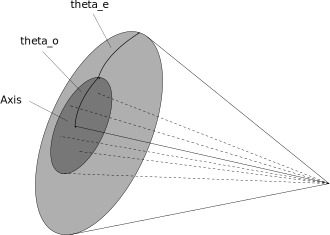
\includegraphics[width=0.3\textwidth]{bounds_o.png}
		\caption{Our internal representation of the Bounds\_o struct}
		\label{fig:boundso}
	\end{center}
\end{figure}

First we will introduce the Bounds\_o struct (\ref{fig:boundso}). This struct represents the orientation bounds of a certain light source or a whole node. For a single light, the axis defines the orientation direction of the light source, while for a node, the axis represents the interpolated axes of all light sources included in the node. Theta\_o defines the maximum angle between the axis of the node and any light source included in this node. Theta\_e defines the additional emission range added to theta\_o for spotlights or area light sources. How we have pictured the geometric representation can be seen in \ref{fig:boundsogeo}. In our implementation, we accept point lights, spotlights and area light sources as light sources. This is how we initialize the Bounds\_o struct for single lights:

\begin{itemize}
	  \setlength\itemsep{0em}
	\item Point light
	\begin{itemize}
		  \setlength\itemsep{0em}
		\item Axis = (1, 0, 0)
		\item theta\_o = $\pi$
		\item theta\_e = $\pi/2$
	\end{itemize}
	\item Spot light
	\begin{itemize}
		  \setlength\itemsep{0em}
		\item Axis = spot direction
		\item theta\_o = 0
		\item theta\_e = spot's apperture
	\end{itemize}
	\item Area light
	\begin{itemize}
		  \setlength\itemsep{0em}
		\item Axis = normal of the geometric representation
		\item theta\_o = 0
		\item theta\_e = $\pi/2$
	\end{itemize}
\end{itemize}

\begin{figure}
	\begin{center}
		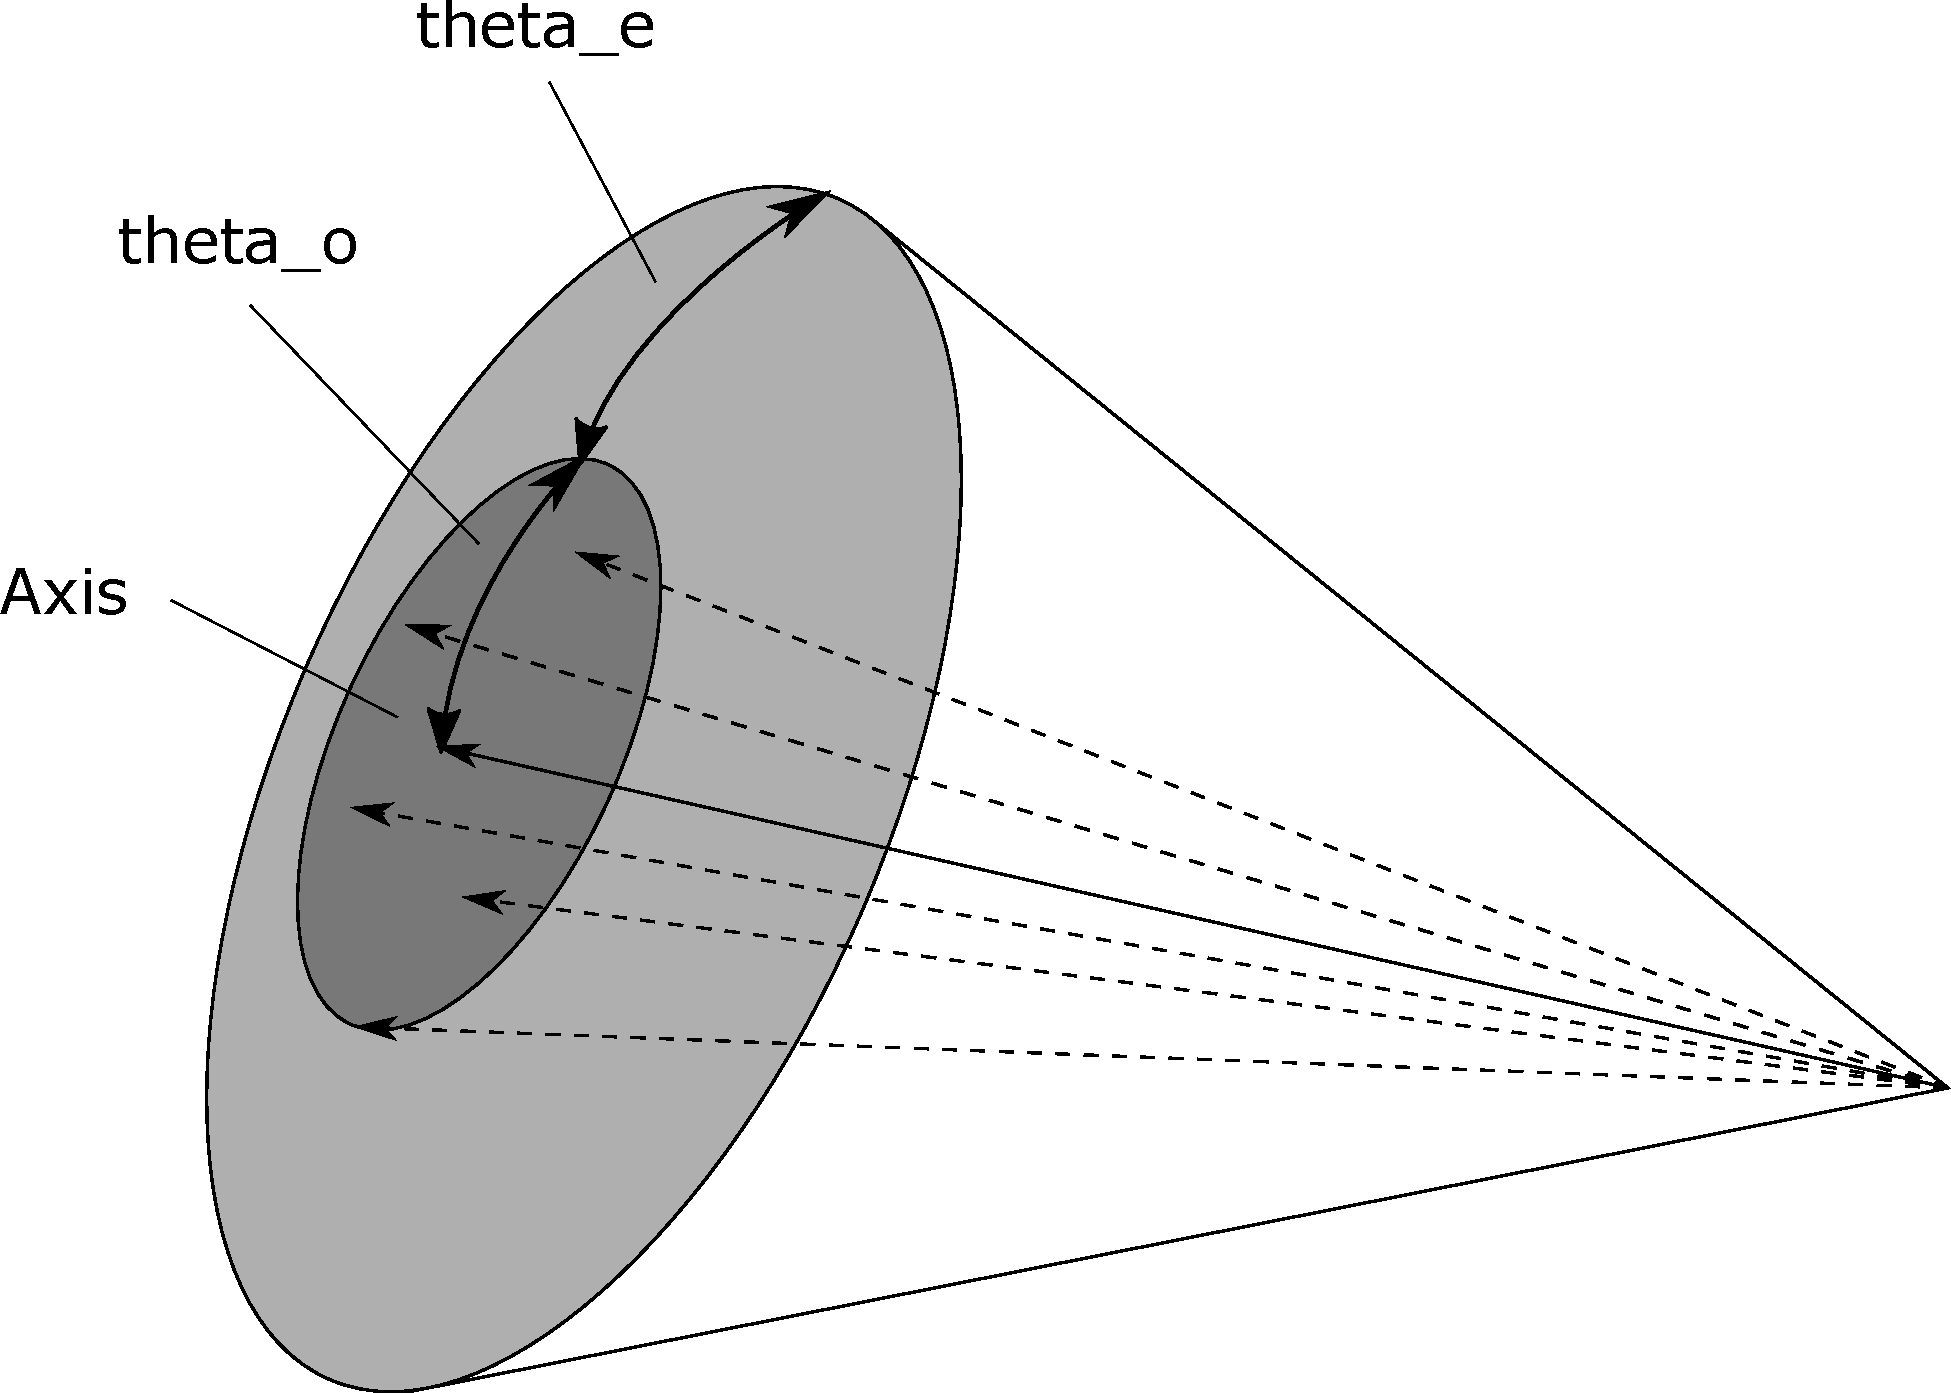
\includegraphics[width=0.6\textwidth]{bounds_o.pdf}
		\caption{geometric idea of the Bounds\_o struct}
		\label{fig:boundsogeo}
	\end{center}
\end{figure}

\subsection{Node representation}

We used two different implementations to represent a node in our light BVH tree (\ref{fig:lightbvhnode} and \ref{fig:linearlightbvhnode}). Both implementations are very similar, containing the two bounding bounds $bounds_w$ for the world space bounds and $bounds_o$ for the orientation bounds, as well as other other information that we will need for the tree traversal later. $Energy$ defines the combined energy of the lights under this node, $nLights$ describes the number of lights under this node, $centroid$ stores the centroid of the world space bounds, and $splitAxis$ stores the coordinate axis that splits the two children of this node. 

The main difference between the two implementations is the way to access the children of the nodes. In our $LightBVHNode$, we have explicit pointers to the two children, while we define the children implicitly in out $LinearLightBVHNode$. Since all of our $LinearLightBVHNodes$ are stored in aligned memory, the way we access the left child is just by incrementing the pointer of the current $LinearLightBVHNode$ by 1. The index needed to access the right child is stored in $secondChildOffset$. To access the second child, we just add $secondChildOffset$ to the base pointer of the root of the tree. If the node is a leaf of the tree and thus only contains one light source, $lightNum$ stores the index of that light source in both implementations.

\begin{figure}
	\begin{center}
		\includegraphics[width=0.5\textwidth]{lightbvhnode.png}
		\caption{Our internal representation of the LightBVHNode struct}
		\label{fig:lightbvhnode}
	\end{center}
\end{figure}

\begin{figure}
	\begin{center}
		\includegraphics[width=0.4\textwidth]{linearbvhnode.png}
		\caption{Our internal representation of the LinearLightBVHNode struct}
		\label{fig:linearlightbvhnode}
	\end{center}
\end{figure}

\section{Surface Area Orientation Heuristic}
\label{sec:saoh}

We have mentioned that we use a different splitting heuristic to build our tree as opposed to using the SAH in a BVH. But we do follow a similar main idea to split the primitives (in our case, the lights) parallel to a coordinate axis, which means that we split in world space. Comparable to splitting the BVH with SAH, where the goal is to minimize the cast of traversing a branch combined with the probability of hitting it, we want to minimize the probability of sampling a branch here. Also, instead of only regarding the number of primitives for each branch, we will rather take into account the combined energy of all the light sources of each branch. Equivalently to SAH, we will also include the surface area in our calculations. So while we do split in world space, we will use the orientation bounds, along with the surface area and the energy, to determine the quality of a certain split. In summary, we define the probability of sampling a given cluster $C$ in the surface area orientation heuristic for as:

\begin{equation}
P(C) = M_A(C) * M_\Omega(C) * Energy(C),
\end{equation}

$M_A(C)$ being the surface area of the cluster, $M_\Omega(C)$ being the bounding cone measure. The surface area of a clusters bounding box with length $l$, width $w$ and height $h$ is the sum of its six faces:

\begin{equation}
M_A(C) = 2(lw + wh + hl).
\end{equation}

\begin{figure}
	\begin{center}
		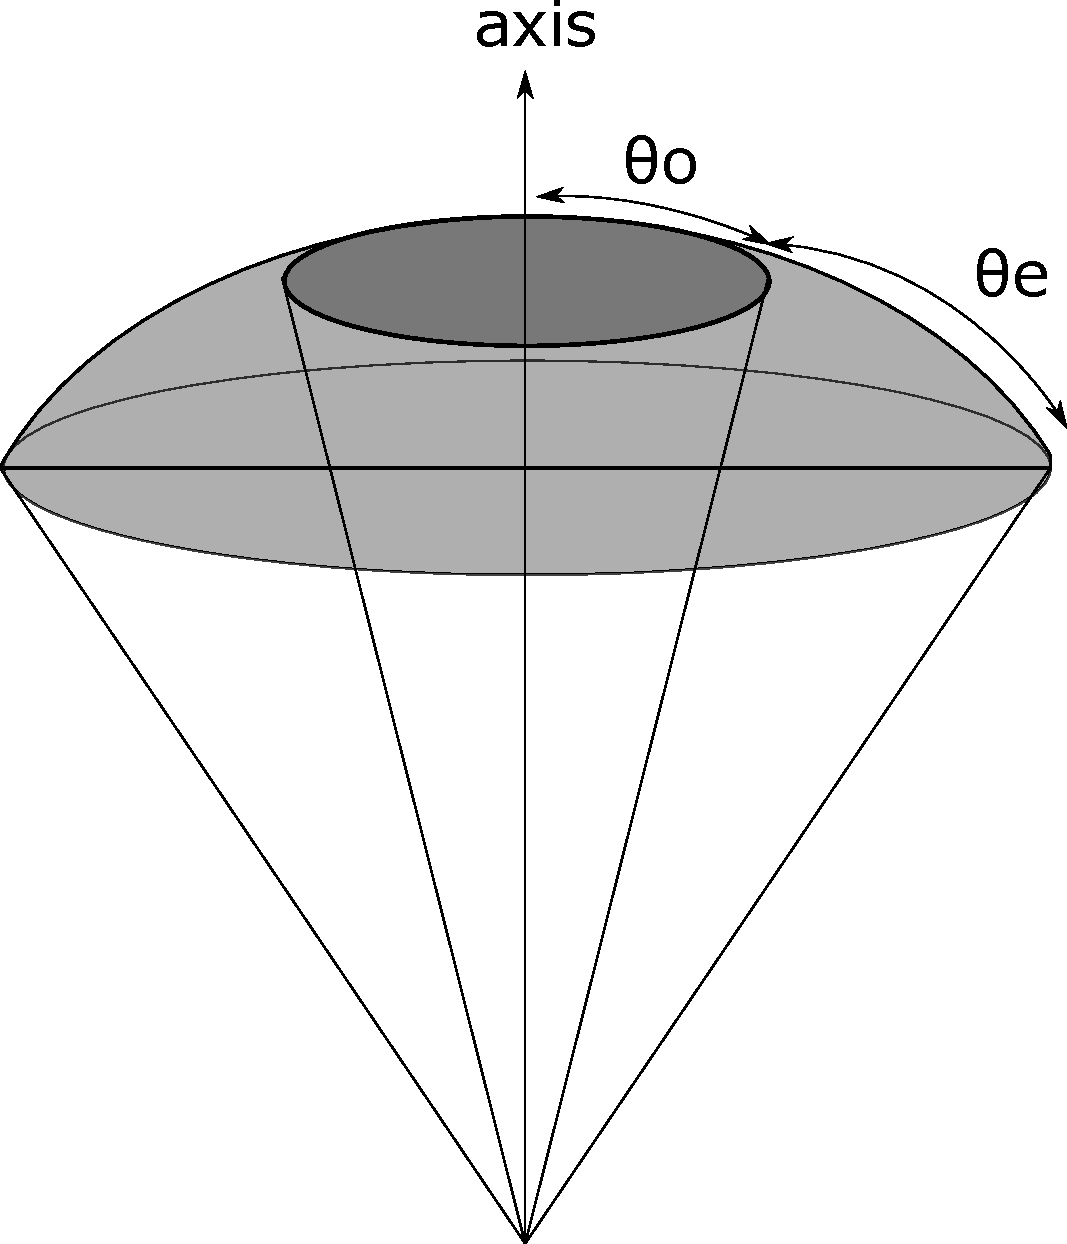
\includegraphics[width=0.4\textwidth]{cone.pdf}
		\caption{Bounding cone measure}
		\label{fig:cone}
	\end{center}
\end{figure}

We used a weighted definition for our bounding cone measure. Remember that we have defined $\theta\_o$ as the bounding angle that encloses the orientation vectors of all the light sources in the cluster, while $\theta_e$ describes their emission range. Obviously, the cone enclosed with $\theta_o$ will most likely have a greater in emission power and thus, we will weight the volume confined by $\theta_o$ with a cosine. A drawing of the individual cones can be seen in \ref{fig:cone}. The measure we have used and has been described in \Cite{MLS} is as follows:

\begin{equation}\label{eq:cone}
M_\Omega(C) = 2\pi * \bigg[(1-\cos(\theta_o)) + \int_{\theta_o}^{\theta_o + \theta_e}\cos(\omega - \theta_o) * sin(\omega)d\omega\bigg]
\end{equation} 

Then, we describe the quality of a split as:

\begin{equation}
c(C_{left}, C_{right}) = \frac{P(C_{left}) + P(C_{right})}{P(C)}.
\end{equation}

Consequently, the quality of a split is inverse to its cost:

\begin{equation}
q(C_{left}, C_{right}) = \frac{1}{c(C_{left}, C_{right})}.
\end{equation}

It is notable that our heuristic tries to find out the possible split in all three dimensions with the given cluster. Therefore, we will try to find the split with the highest quality and split the cluster there.

\begin{figure}
	\begin{center}
		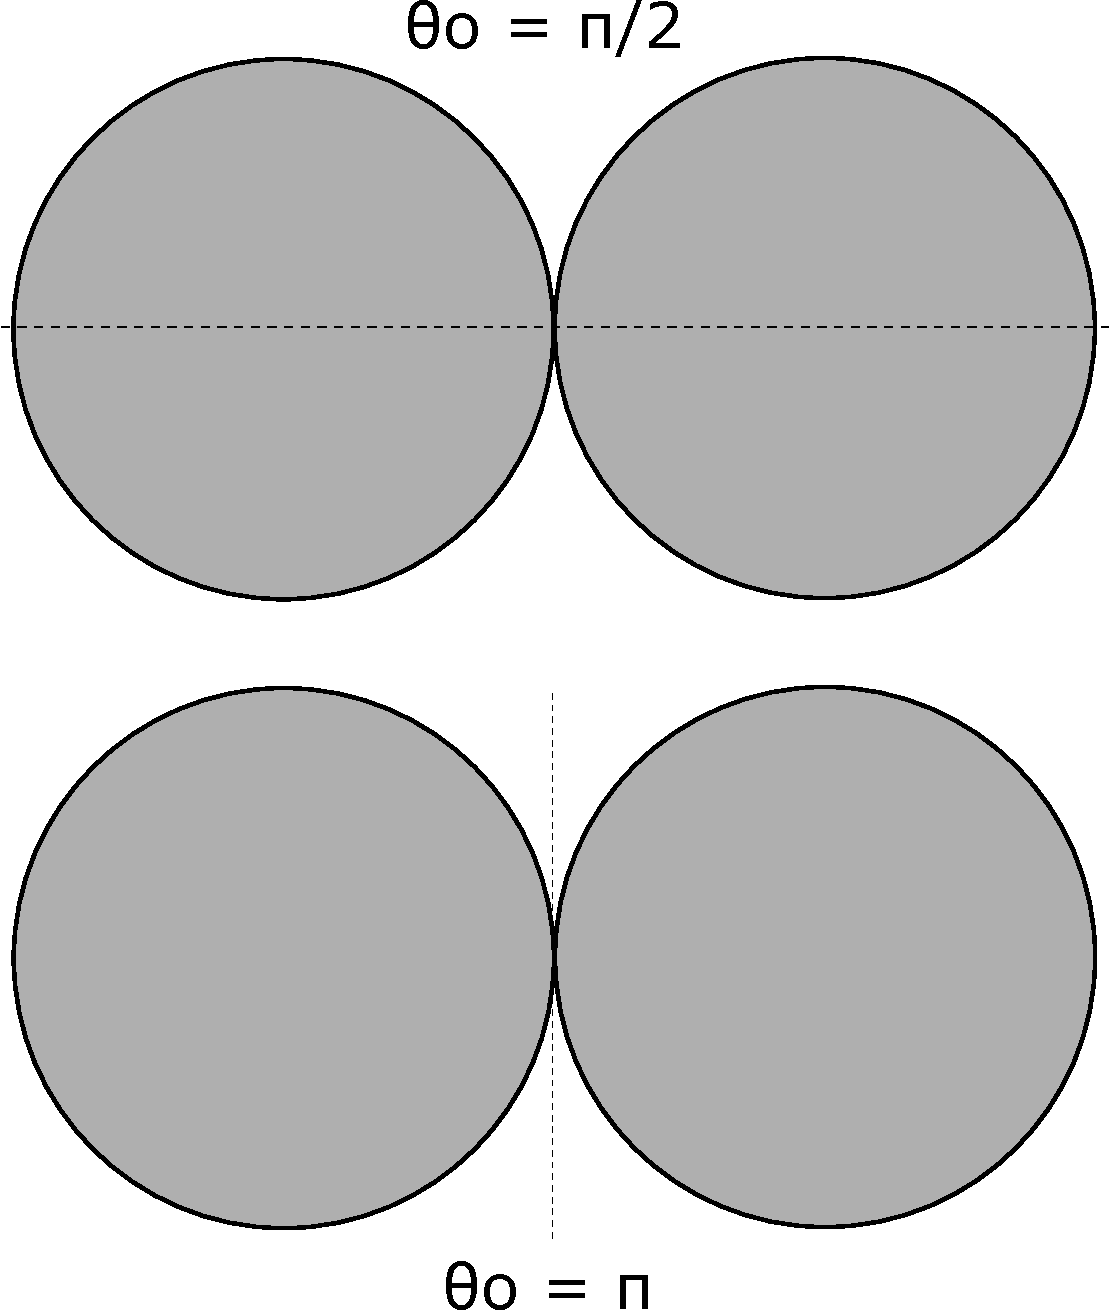
\includegraphics[width=0.5\textwidth]{idealsplit.pdf}
		\caption{Preferred split example}
		\label{fig:idealsplit}
	\end{center}
\end{figure}


Now, what does our heuristic exactly do for specific clusters? The general idea is that we try find splits in a way that the orientation cones of both children are as focused as possible. Suppose we have a great number of small triangle emitters that shape up together as two spheres like modelled in \ref{fig:idealsplit}. Obviously, the normals of the triangle emitters of a single sphere point to all possible directions in the scene. If we would have a cluster containing every single triangle emitter of the two spheres, our $\theta_o$ value of that cluster would be $\pi$; the normals over the unit sphere of $2\pi$ or 360°. Making the bottom split which splits the two spheres would result in not much change: The axis of the emitters would still cover every possible direction and the $\theta_o$ values of both children would still be $\pi$. In this case, we would definitely prefer the top split that splits both spheres in half, resulting in the normals over covering half of the unit sphere. We reduced $\theta_o$ to $\pi/2$. SAH alone would have not told the difference between those two splits and that's why the bounding cone measure is a very integral part of our cost calculation algorithm

\section{Light Bounding Volume Hierarchy Construction}
\label{sec:alg:con}

In this section we will be talking about our in-depth implementation of the tree construction. The tree constructor method takes two parameters. First, a vector containing all the light sources in the scene. Second, we will take a parameter defining the split threshold that describes if we want to sample multiple light sources when traversing the light BVH later (\ref{subs:split}). The split threshold is a normalized value between 0.0 and 1.0. A split threshold of 1.0 never splits, we would only shade one light per point and a split threshold of 0.0 always splits, which means all lights of the scene are shaded. Note that our algorithm is implemented to work with any combination of point light sources, area light sources and spotlights.

\begin{algorithm}
	\caption{LightBVHAccelerator constructor}
	\label{LightBVHAccelerator}
	\begin{algorithmic}[1] % The number tells where the line numbering should start
		\Procedure{LightBVHAccel}{vector<Light> \&lights, float splitThreshold}
		\State $LightBVHNode \; *root  \gets recursiveBuild(lights, 0, lights.size());$
		\State $LinearLightBVHNode \; *nodes \gets AllocAligned(totalNodes);$ 
		\State $flattenLightBVHTree(nodes, root, 0);$
		\EndProcedure
	\end{algorithmic}
\end{algorithm}

The $lightBVHAccel$ constructor initializes the tree construction. First, we will be using a recursive approach to build the light BVH. We will pass the light sources of the scene in an array and the starting and ending indices of the current node, obviously for the root of the light BVH we will pass the whole range of our vector. Then, after we have constructed our tree represented by $LightBVHNode$ objects, we will flatten the tree in a compacter form represented by $LinearLightBVHNode$ objects to ensure that our tree requires as little memory as possible and to improve cache locality. $Nodes$ will later be our object to run our tree traversal on.

\begin{algorithm}
	\caption{LightBVHAccelerator recursive build}
	\label{recursiveBuild}
	\begin{algorithmic}[1] % The number tells where the line numbering should start
		\Procedure{LightBVHNode* recursiveBuild}{vector<Light> \&lights, int start, int end}
		\State LightBVHNode *node;
		\If{end - start == 1}
			\State *node = $initLeaf()$;
			\State \Return node;
		\EndIf
        \ForEach {\texttt{dimension}}
        	\State <calculate axis and thetas for the whole node for current dimension>
			\State <calculate all split costs for current dimension>
		\EndFor
		\State <find out best split>
		\State <initialize child nodes and make reference as children>
		\State \Return node;
		\EndProcedure
	\end{algorithmic}
\end{algorithm}

Our recursive implementation of the light BVH construction take a vector including all lights of the scene, as well as start and end indices for the current node. The implementation can be split into multiple sections. Obviously, we want to cover the base case first, when we only have a single light source under the node. In this case, we cannot split further, so we will just initialize a leaf node with the one light source and return this leaf node. Next, we will be calculating the axis and $\theta$ values for the whole node for all three dimensions. This is required for the split cost calculations for every split in the current dimension we are working on. After we have computed the split qualities for every individual split in all dimensions, we will find out the best possible split among these we have calculated and initialize the left and right child, which we will reference as children of the current node.

The reader may have already realized that our implementation is very close to popular implementations of BVH constructions; that makes sense since our implementation was heavily influenced by BVH constructions the structure of our tree is analogical to that of BVHs. It should be also noted that we count the number of nodes we create. This number is required for the flattening of our tree later (\ref{subs:flat}).

\subsection{Axis Calculation}
\label{subs:axis}

\begin{figure}
	\begin{center}
		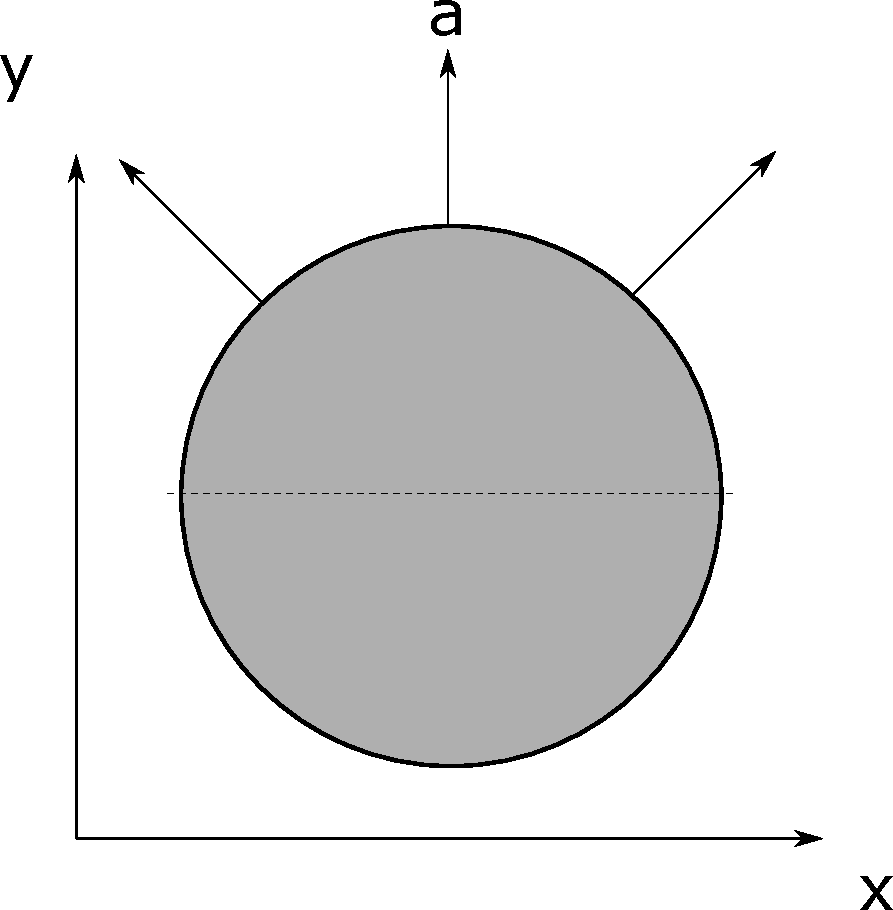
\includegraphics[width=0.5\textwidth]{axis.pdf}
		\caption{Axis calculation}
		\label{fig:axis}
	\end{center}
\end{figure}

Next, we will do axis calculations for the whole cluster for a specific dimension. We have tried two different approaches for the axis calculations. Our first approach used the median of the individual axes of all lights included in the cluster sorted by the specific dimension we are working on. So, if we wanted to find out the qualities of the individual splits if we split the lights at a particular x-coordinate, we would take the axis of the median light if we sorted them according the x-coordinate of their axes. This approach leads to a major problem. Since our geometric representation is three-dimensional, taking the median axis sorted by a single dimension does not always represent the ideal axis that we are looking for. Suppose we have a scene as modelled in \ref{fig:axis} and suppose we have chose to split the sphere in half along the axis y. Like previously discussed in \ref{fig:idealsplit}, the axis of our hemisphere should be $a$ or at least close to $a$. Calculating the cluster axis like just described would result to a very different and unexpected result. Instead of finding $a$ as the axis, instead, we would find one of the other two axis plotted in the image. Those are the two median axis if you sort the axis of the individual emitters according to their y-value. It is evident, that this approach does not archive the desired results. 

\begin{figure}
	\begin{center}
		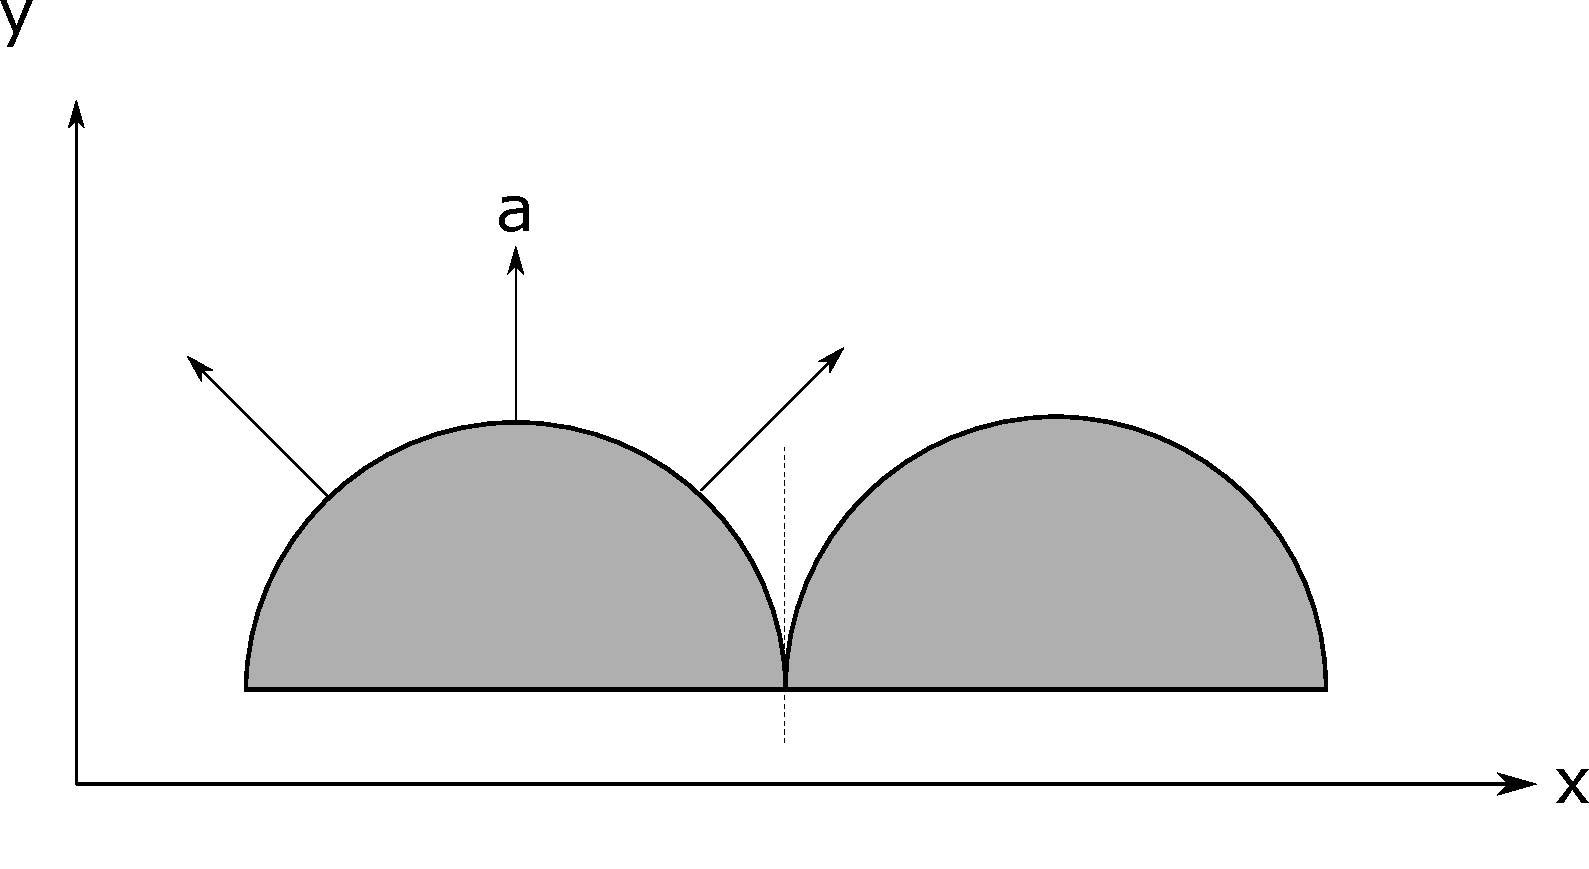
\includegraphics[width=0.8\textwidth]{axis2.pdf}
		\caption{Axis calculation}
		\label{fig:axis2}
	\end{center}
\end{figure}


Using the median axis sorted by another coordinate value works in this example, but does not yield the correct results in general either. Suppose we already have hemispheres like in \ref{fig:axis2} and the split you can see in the drawing. In this situation, we would actually want to use the median axis sorted by the x-coordinate after having split along the axis x. Sorting by the y-values would lead to unwanted results. As you can see, only considering the value of one of the dimensions of the axes is not enough; instead we have to regard all the three dimensions. Our second approach that we are using now deals with this problem properly. Instead of using the median axis, we use the average or the normalized sum of the individual axes of all light sources in the cluster:

\begin{equation}
C_{axis} = \frac{\sum_{i = 0} a_i}{|\sum_{i = 0} a_i|},
\end{equation}

with $a_i$ being the axis of the i-th light source in the cluster. This axis definition for a cluster eliminates the problem presented in \ref{fig:axis}. Both median and average calculations have $O(n)$ time complexity, but especially in scenes with symmetric objects that represent light sources, our current approach leads to much better results.

\subsection{Theta Calculations}
\label{subs:theta}

\begin{algorithm}
	\caption{Theta calculations}
	\label{thetacalculations}
	\begin{algorithmic}[1] % The number tells where the line numbering should start
		\Procedure{calculateThetas}{vector<Light> \$lights, 3DVector axis, float *theta\_o, float *theta\_e}
		\For{\texttt{int i = 0; i < vector.$size$(); i++}}
			\State Light l $\gets$ lights[i];
			\State float current\_o $\gets$ 0.f;
			\State float current\_e $\gets$ 0.f;	
			\State 	*theta\_o $\gets$ $max$(*theta\_o, $radianAngle$(axis, l.axis) + l.theta\_o);
			\State *theta\_e $\gets$ $max$(*theta\_e, o + l.theta\_e);
		\EndFor
		\State *theta\_e -= *theta\_o;
		\State *theta\_e $\gets$ $min$(*theta\_e, $\pi$ - *theta\_o);
		\EndProcedure
	\end{algorithmic}
\end{algorithm}

We have listed our the calculations for $\theta_o$ and $\theta_e$ in \ref{thetacalculations}. The procedure takes the base address of a vector containing of the lights that define the specific cluster, as well as the axis of the cluster. Also, pointer to two floats are passed to return the $\theta$-values. The calculations made are very simple; we iterate through the lights that were passed to us and calculate the individual $\theta_o$ and $\theta_e$ values of the given axis with the axis of the whole cluster. If any of the $\theta$ values are greater than the current maximum $\theta$ values we have stored, we update our maximum $\theta$ values. At the end, when we have processed all light sources, we have to first subtract $\theta_o$ from $\theta_e$ as we only store the additional angle to $\theta_o$ in $\theta_e$. Next, we will also need to limit $\theta_e$ with $\pi - \theta_o$, otherwise it is possible to get a negative integral in our bounding cone measure \ref{eq:cone}. This is something we want to avoid because the measured volume of the bounding cone should always be non-negative.

\subsection{Buckets}
\label{subs:buckets}

Before we jump into our split cost implementation, we want to talk about a design decision we made. The first approach we tried was to split the light sources after every single light source, which means, if we had 1.000 lights, we would have 999 different splits in each dimension. We realized that this approach does not scale well for very large amounts of light sources. We measured the time for building the light BVH on different scenes with varying amounts of emitters on a computer with a Intel® Core™ i7-4770K processor and 16 gigabyte of main memory. For instance, a scene with 10.000 emitters works just fine with a rendering time of TODO. On the other hand, the tree construction time of another scene with one million light sources takes TODO. Obviously, this construction time is way too long and not useful for practical uses. 

Therefore, we decided to use specific amounts of buckets that determine the position where we split the light sources. At the start, we will define a maximum amount of splits that we want to calculate for any cluster. What has worked well for us is to calculate a maximum number of 10.000 splits. This way, we have an acceptable rendering time of TODO for the scene with one million light sources, while the split quality stays roughly the same like if we would calculate every possible split. When we have settled on $b$, the amount of buckets to use, we will define the number of light sources in each bucket as:

\begin{equation}
n = \frac{b}{N},
\end{equation}

with $N$ being the total number of emitters of the cluster. Then, we will split the lights of the cluster at the indices that are multiples of $n$, resulting to $b$ different splits. 

\begin{figure}
	\begin{center}
		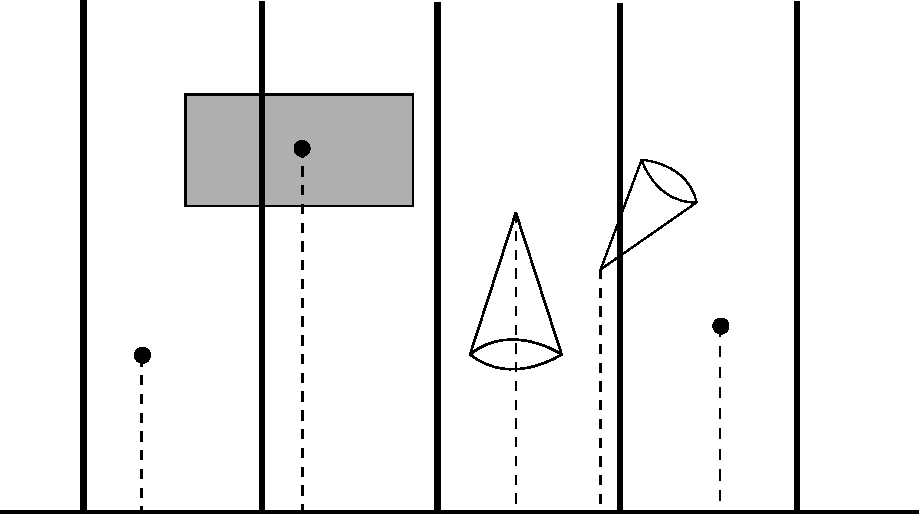
\includegraphics[width=0.6\textwidth]{bucket.pdf}
		\caption{Bucket splits for area light sources, point light sources and spotlights}
		\label{fig:bucket}
	\end{center}
\end{figure}

Another approach to split the scene in multiple buckets is to split the world space coordinates for a specific dimension into equally big areas and projecting the centroid value of the light sources on the coordinate plane of that dimension. The general idea can be seen in \ref{fig:bucket}. So, instead of splitting after a certain amount of emitters, we split after a definite chunk of world space. The difference between these two ideas was not huge, but we decided to stick to splitting after a fixed number of emitters because especially in scenes, where the emitters are focused in a small area, this approach seemed to make more sense.

\subsection{Split Cost Calculation}
\label{subs:splitcost}

\begin{algorithm}
	\caption{Split Cost Calculation}
	\label{alg:splitcostcalculation}
	\begin{algorithmic}[1] % The number tells where the line numbering should start
		\Procedure{int[] calculateCost}{vector<Light> \$lights, int buckets}
		\State float[buckets] cost;
        \ForEach {\texttt{split i}}
		\State <calculate axis, thetas, AABB and energy for the left part>
		\State <calculate axis, thetas, AABB and energy for the right part>
		\State <calculate leftCost, rightCost and totalCost>
		\State cost[i] $\gets$ (leftCost + rightCost) / totalCost;
		\EndFor
\State \Return cost;
\EndProcedure
\end{algorithmic}
\end{algorithm}

First, we have to sort the light sources by their coordinate value of the current dimension we are working on, since we split in world space. Then, we use the previously discussed buckets to determine positions where to split the emitters. For each individual split, we will be doing axis, theta and AABB as described in \ref{subs:axis}, \ref{subs:theta} and \ref{sec:aabb}. The total energy of a cluster is simply the sum of the energy values of the individual light sources. Afterwards, we will do the cost calculations for the left part, the right part and the total cluster according to \ref{sec:saoh}. The split cost of this bucket is then stored in the respective entry of cost. After we have iterated through all the buckets for this particular dimension, we will return the array containing all split values of this dimension.

\subsection{Choosing the best split}

There is not much to talk in this subsection. We iterate through the arrays containing the cost values of each individual split and choose the split with the lowest cost value, i.e. the split that has the highest quality. Depending on the implementation and if we use buckets, we have to calculate the index where we split our cluster and perhaps the dimension of the split.

\subsection{Creating the children nodes}

\begin{algorithm}
	\caption{Children creation}
	\label{alg:childrencreation}
	\begin{algorithmic}[1] % The number tells where the line numbering should start
		\Procedure{LightBVHNode* createChildren}{vector<Light> lights, int splitIndex, int splitDimension}
		\State $partialSort$(\$lights, splitIndex, splitDimension);
		\State LightBVHNode *leftNode $\gets$ $recursiveBuild$(lights, 0, splitIndex + 1);
		\State LightBVHNode *rightNode $\gets$ $recursiveBuild$(lights, splitIndex + 1, lights.$size$());
		\State node $\gets$ $initInterior$(leftNode, rightNode);
		\State \Return node;
		\EndProcedure
	\end{algorithmic}
\end{algorithm}

At this point, we have found out the dimension of our optimal split, as well as the index where to split our cluster. Our first step is to make a partial sort at the split index with individual lights of the cluster. We have to sort according to the centroids world space coordinates of the given dimension. That makes sense, since our primary goal was the split the cluster in world space and use the orientation solely for split cost calculations while constructing the tree. Afterwards, we recursively call $recursiveBuild$ with the indices for the left and the right child and make references of the children in our parent node.

\subsection{Tree Flattening}
\label{subs:flat}

\begin{algorithm}
	\caption{Tree flattening}
	\label{alg:treeflattening}
	\begin{algorithmic}[1] % The number tells where the line numbering should start
		\Procedure{int flattenLightBVHTree}{LinearLightBVHNode *nodes, LightBVHNode *node, int *offset}
		\State LinearLightBVHNode *linearNode $\gets$ \&nodes[*offset];
		\State linearNode.$copy$(node);
		\State int myOffset $\gets$ (*offset)++;
		\If{node->nLights == 1}
		\State linearNode->lightNum $\gets$ node->lightNum;
		\Else
		\State linearNode->splitAxis $\gets$ node->splitAxis;
		\State $flattenLightBVHTree$(nodes, node->children[0], offset);
		\State linearNode->secondOffset $\gets$ \\ \ \ \ \ \ \ \ \ \ \ \ \ \ \ \ \ \ $flattenLightBVHTree$(nodes, node->children[1], offset);
		\EndIf
		\State \Return myOffset;
		\EndProcedure
	\end{algorithmic}
\end{algorithm}

We have a representation of all light sources of the scene in a binary tree now and at this point, we say that we are finished with our tree construction and use this tree as the acceleration data structure to do the sampling on. At first, we did exactly that and did not bother to flatten the tree. But when traversing the tree, we have realized that the nodes were not ordered in a linear way in our memory. That leads to more cache misses, worse memory usage and just worse performance overall, which is why we looked for a way to change this aspect of our light BVH representation. We chose to use a implementation that uses a contiguous chunk of memory. How we modelled a single node in our code can be seen in \ref{fig:linearlightbvhnode}. The general idea is that the left child node is implicitly referenced because it is stored as the next child in the memory. Therefore, we only need to store the offset to the right child of each interior node explicitly. The pseudo code of our implementation can be seen in \ref{alg:treeflattening}. Remember that we call this method on the root of our light BVH tree before flattening with the base address of our pre-allocated memory passed in $*nodes$ (\ref{LightBVHAccelerator}) The offset passed is obviously 0 at the beginning.

The function returns the offset for the current node we are working on. First, we will creating a $LinearLightBVHNode$ at the address given by $\&nodes + offset$ and will be copying the data from $*node$ that are used for all nodes, regardless if the node is an interior node or a leaf node. That includes:

\begin{itemize}
	\item World space bounds
	\item Orientation bound
	\item Energy of the node
	\item Centroid of the node
	\item Number of emitters under this node
\end{itemize} 

After incrementing the offset, so $\&nodes + offset$ points to the address where the next $LinearLightBVHNode$ should start, we will be dealing with two cases: Either the currently regarded node is a leaf node or an interior node. If the node is a leaf node, all we need to do is set the light number are finished. If the node is an interior node, the splitAxis need to be set and we will have to call the method recursively for the left and the right child, while storing the offset returned by the second child as the $secondChildOffset$. That will be our explicit reference to the second child when traversing the tree later.

\begin{figure}
	\begin{center}
		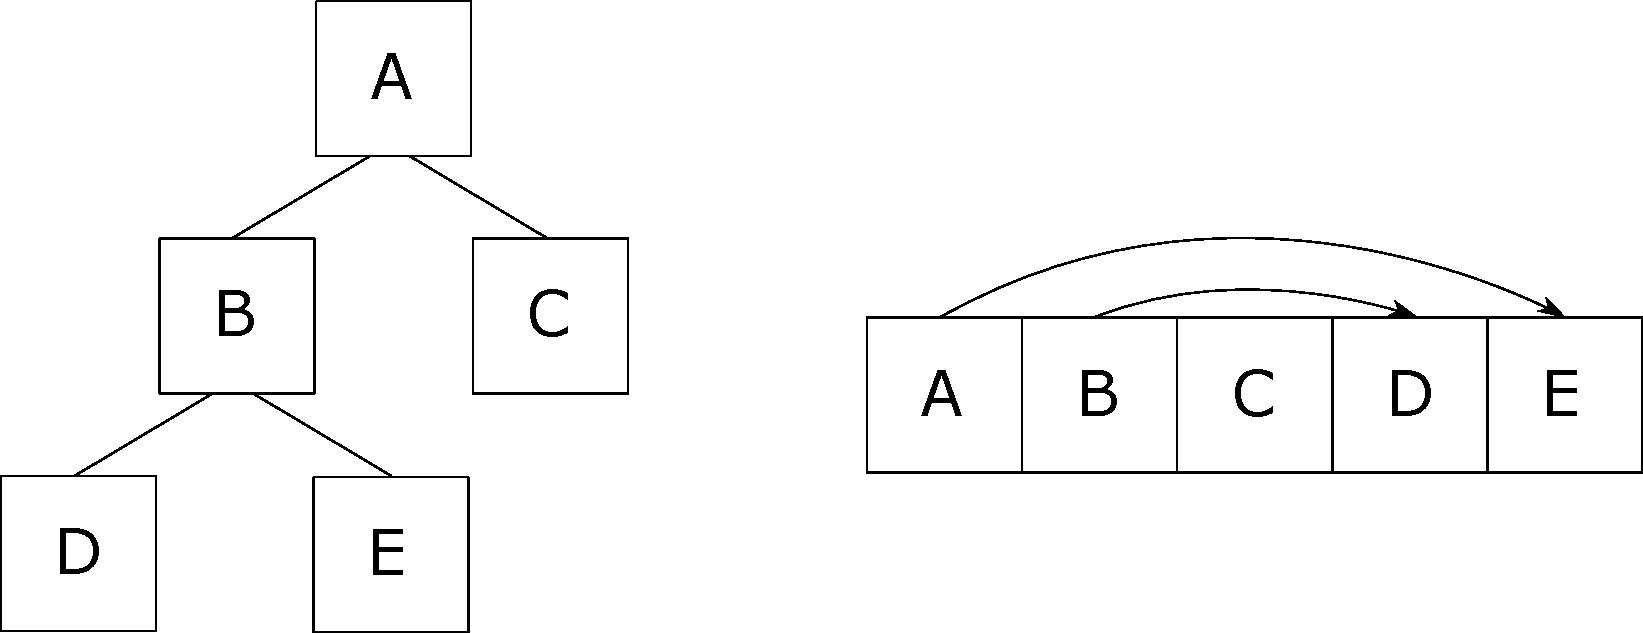
\includegraphics[width=0.8\textwidth]{flattening.pdf}
		\caption{Tree representation before and after flattening}
		\label{fig:flattening}
	\end{center}
\end{figure}

The effect of calling this method on the root of the light BVH tree can be seen in \ref{fig:flattening}. Suppose we have a very simple tree with only five total nodes consisting of two interior nodes (A and B) and three leaf nodes (C, D and E) like in the drawing. In our pre-flattened version of our light BVH, the nodes do not necessarily need to be in a contiguous chunk of memory. Instead, every interior node would have references to two child nodes. After the flattening, the nodes are ordered in a linear way in a coherent chunk of memory. The left child is implicitly referenced by the next node in the memory and the right child can be referenced via an offset. In our example, the left child of A is implicitly referenced by the next node in memory, as well as the left child of B. The right child can be found with the sum of the offset and the base address. Obviously, with the non-linear implementation, our cache, memory and overall system performance could be extremely lacking in worst cases and will definitely be worse in average cases than our flattened version.

\section{Light Bounding Volume Hierarchy Traversal}
\label{sec:alg:tra}

We have successfully constructed an acceleration data structure for our light sampling problem. The next step will be obviously doing the tree traversal. If we think back to \ref{sec:preliminaries:pat}, in our light transport equation we have two different functions in the integrand. 

\begin{equation}
L_o(p, \omega_o) = \int_{\varsigma^2}f(p, \omega_o, \omega_i)L_d(p, \omega_i)|cos\theta_i|d\omega_i
\end{equation}

Both function can be sampled with Monte Carlo integration and while $f(p, \omega_o, \omega_i)$ depends on the BSDF of the material of the intersection point, $L_d(p, \omega_i)$ can be importance sampled when we choose an emitter that has a big contribution to the intersection point. Our goal, in summary, is to return light sources that have a high contribution to the intersection point more often. In most cases that would be done by creating a distribution that has a similar form to that of $L_d(p, \omega_i)$, but in our situation, that is not practicable. Calculating a distribution for every single new intersection point would not make a lot of sense since these distribution cannot be reused. In special scenes, we might sample light sources for a single point multiple times, but in general that will not be the case. Instead of generating distributions, we will make a decision at every branch of our tree to go left or right based on a random number.


\begin{algorithm}
	\caption{Sampling a single light source}
	\label{alg:sample1}
	\begin{algorithmic}[1] % The number tells where the line numbering should start
		\Procedure{int sampleOneLight}{Intersection \&it, float *pdf}
			\State float sample1D $\gets$ $UniformFloat()$;
			\State *pdf $\gets$ 1;
			\State \Return $TraverseNodeForOneLight$(nodes, sample1D, it, pdf);
			\EndProcedure
		\end{algorithmic}
	\end{algorithm}
	
	\begin{algorithm}
		\caption{Sampling multiple light source}
		\label{alg:sample2}
		\begin{algorithmic}[1] % The number tells where the line numbering should start
			\Procedure{vector<pair<int, float>> sampleMultipleLights}{Intersection \&it}
				\State vector<pair<int, float>> lightVector;
				\State $TraverseNodeForMultipleLights$(nodes, it, \&lightVector);
				\State \Return lightVector;
				\EndProcedure
			\end{algorithmic}
		\end{algorithm}

Our implementation offers two functions to call to sample a light source when passing an intersection point. The two functions are $SampleOneLight$ when not splitting and $SampleMultipleLights$ when splitting. The main reason for two different functions for a functionality that could be provided by a single function is that we want to avoid unnecessary work if possible. When sampling multiple lights, it is required to return a data structure that stores a collection of references to the emitters. That is not mandatory for sampling a single light source. Since this method is called every time we want to sample a light source, the additional overhead can add up to a substantial amount of extra rendering time. Our two implementations of the sampling functions can be seen in \ref{alg:sample1} and \ref{alg:sample2}. There are a few things to point out in our implementation. First, note that $nodes$ is a pointer to our root of our flattened tree and is a private member of our tree representation. Second, the $Intersection$ to be passed stores information about the intersection point, including its world space position, as well as its normal and BSDF representation. That is required for splitting and optimization later. Third, additionally to the number of the light source, we return a value of the probability density function (PDF) in both sampling functions. As we have explained in earlier sections, this is an integral part of importance sampling that cannot be skipped. When sampling a single light source, we generate a uniform random number between 0 and 1 and make branch decisions based on that number. This step is postponed when sampling multiple light sources for two different reasons. It is not required at this point and we want to draw a uniform random number for each light source to sample instead of using a single uniform random number. Instead, we will initialize a vector that will later be filled with the index numbers of the sampled light sources and their respective PDFs. Lastly, we have to mention an important detail about the return of these functions. In some cases, when traversing through the light BVH, it will be already evident, that not a single emitter in the branch we are current traversing though will have a contribution to the intersection point. In these situations, we will return -1 to signal that we did not sample a light.

\subsection{Sampling a single light source}
\label{subs:single}

\begin{algorithm}
	\caption{Sampling a single light source}
	\label{alg:sample1}
	\begin{algorithmic}[1] % The number tells where the line numbering should start
		\Procedure{int TraverseNodeForOneLight}{LinearLightBVHNode *node, Intersection \&it, float *pdf}
		\If{node->nLights == 1}
		\State \Return node->lightNum;
		\EndIf
		\State float left $\gets$ calculateImportance(it, \&node[1]);
		\State float right $\gets$ calculateImportance(it, nodes[node->secondChildOffset]);
		\State float total $\gets$ left + right;
		\If{total == 0}
		\State \Return -1;
		\EndIf
		\State left /= total;
		\State right /= total;
				\State <branch according to importance and sample1D>
		\EndProcedure
	\end{algorithmic}
\end{algorithm}

We will be talking about how we traverse through the light BVH when sampling a single light source in this subsection. First, we cover the base case when we already arrived at a leaf node of our tree representation. In this case, we have reached a node that contains only a single light source which represents the sampled light source. We simply return the index of the emitter stored in the current node, as well as the PDF that has been calculated while traversing through the tree.

If we are currently in an interior node, we will have to calculate the importance values for both children. The left child is simply the next node in memory, while we will reference the right child explicitly with the $secondChildOffset$ of the current node. Then, we will normalize these importance values and check if their sum is zero. In this case, the current node we are working on, will have no contribution to the intersection point and we will return -1. If the total value is non-zero, we will make a decision to go left or right based on the importance values and the uniform random number we drew earlier.

\subsection{Splitting}
\label{subs:split}
	%% LaTeX2e class for student theses
%% sections/evaluation.tex
%% 
%% Karlsruhe Institute of Technology
%% Institute for Program Structures and Data Organization
%% Chair for Software Design and Quality (SDQ)
%%
%% Dr.-Ing. Erik Burger
%% burger@kit.edu
%%
%% Version 1.3.3, 2018-04-17

\chapter{Evaluation}
\label{ch:Evaluation}

%% -------------------
%% | Example content |
%% -------------------
\dots

\section{First Section}
\label{sec:Evaluation:FirstSection}

\dots

\section{Second Section}
\label{sec:Evaluation:SecondSection}

\dots

\section{Third Section}
\label{sec:Evaluation:ThirdSection}

\dots
%% ---------------------
%% | / Example content |
%% ---------------------
	%% LaTeX2e class for student theses
%% sections/evaluation.tex
%% 
%% Karlsruhe Institute of Technology
%% Institute for Program Structures and Data Organization
%% Chair for Software Design and Quality (SDQ)
%%
%% Dr.-Ing. Erik Burger
%% burger@kit.edu
%%
%% Version 1.3.3, 2018-04-17

\chapter{Related Work and Future Work}
\label{ch:related}

\section{Lightcuts}

Lightcuts \Cite{LCT} tried to deal with the same problem as we did very early on in 2005. In scenes with complex illumination with many light sources, Lightcuts tries to approximate the direct lighting by substituting a cluster of lights by a single representational light source. So, in situations, where we would want to illuminate an intersection point with every light source in the scene, we can instead illuminate the point with a smaller subset of light sources. That leads to a model that scales much better with many light sources in the scene.

The basic algorithm follows a simple concept that can be divided into certain steps:

\begin{itemize}
	\item Convert illumination to point lights
	\item Build light tree
	\item For each eye ray, choose a cuts to approximate the illumination
\end{itemize}

We will break down the single steps for the reader. First, the complex illumination of the scene is substituted by point lights with a similar lighting. The reason for that is that the algorithm required point lights to run. Next, a binary tree that includes every emitter of the scene is built, with the interior nodes representing light clusters and the leafs representing single emitters. When rendering, for each eye ray, the algorithm calculates a cut that minimizes the number of lights sampled, while guaranteeing a certain quality threshold. A cut of the binary tree is a substitution of the total number of emitters in the scene. Either, the cut includes the actual light source or a cluster as a substitution of said light source. Therefore, when we light a intersection point with a cut, we limit the number of sampled lights.

To find out a suitable cut for an eye ray, the algorithm will start with the cluster that substitutes the whole lighting of the scene with a certain light. Gradually, the algorithm will increase the number of representative lights, as long as the quality of the lighting would increase over a certain threshold. If none of these substitutions will yield us a noticeable increase in quality, we will stop the algorithm and work with the cut calculated.

The paper further introduces reconstruction cuts, that calculates the color of certain positions sparsely over the image and then interpolates their illumination to shade the rest of the image.

While lightcuts are a interesting approach to dealing with scenes with complex illumination, while path tracing, we would have to calculate much more cuts to illuminate the scene. Also, due to it's approximating nature, the rendered image will never converge to the ideal image.

\section{Importance Sampling of Many Lights with Adaptive Tree Splitting}

The contribution of Conty and Kulla \Cite{MLA,MLS} was basically the source of the idea for this algorithm. Many of the things we have explained has been implementated the same way or similarly in their works. We have marked the spots in this thesis where we drastically changed our algorithm compared to their ideas. In the scenes we have tested our version of the algorithm, the images appear less noisy. Sadly, our splitting algorithm could not meet the qualities of the quality they have described in their presentation.

\section{Future Work}

As we have mentioned in the previous section, our splitting algorithms does not have the desirable quality. Obviously, that is the first thing we want to improve. Being able to archive a higher quality with a shorter rendering time is just what this thesis is about.

Next, we would like to be able to use our algorithm in scenes that are not only lighted by point lights, spotlights and area light sources. For instance, we would like to implement distant light sources like the illumination of the sun or projection light sources that model the lighting of a slide projector.

Finally, at some points we have tried optimized our algorithm, for instance by creating a more compact data structure for a faster tree traversal. On other points, we have favored keeping the code in a more readable state instead of optimizing it for development reasons. When we are sure that we will not change too much in our implementation anymore, it would clearly be desirable to optimize the code for a faster rendering time.
	%% LaTeX2e class for student theses
%% sections/conclusion.tex
%% 
%% Karlsruhe Institute of Technology
%% Institute for Program Structures and Data Organization
%% Chair for Software Design and Quality (SDQ)
%%
%% Dr.-Ing. Erik Burger
%% burger@kit.edu
%%
%% Version 1.3.3, 2018-04-17

\chapter{Conclusion}
\label{ch:Conclusion}

\dots
	
	%% --------------------
	%% |   Bibliography   |
	%% --------------------
	
	%% Add entry to the table of contents for the bibliography
	\printbibliography[heading=bibintoc]
	
	%% ----------------
	%% |   Appendix   |
	%% ----------------
	\appendix
	
\end{document}